\documentclass{article}
\setlength{\parskip}{5pt} % esp. entre parrafos
\setlength{\parindent}{0pt} % esp. al inicio de un parrafo
\usepackage{listings} % listings
\usepackage{color} %colores
\usepackage{amsmath} % mates
\usepackage[sort&compress,numbers]{natbib} % referencias
\usepackage{url} % que las URLs se vean lindos
\usepackage[top=15mm,left=20mm,right=20mm,bottom=25mm]{geometry} % margenes 
\usepackage{hyperref} % ligas de URLs
\usepackage{graphicx} % poner figuras
\usepackage[spanish]{babel} % otros idiomas


\author{Claudia Lizeth Hern\'andez Ram\'irez} % author
\title{Homework 1 - Algoritmo Gen\'etico} % titulo
\date{\today}

\definecolor{mypurple}{rgb}{0.305, 0.066, 0.592}
\definecolor{mygray}{rgb}{0.976, 0.980, 0.980}
\definecolor{myorange}{rgb}{0.933, 0.305, 0.090}
\lstset{ 
  backgroundcolor=\color{mygray},
  commentstyle=\color{myorange},
  keywordstyle=\color{mypurple}, 
  numberstyle=\tiny\color{myorange}
  stringstyle=\color{mypurple}, 
  breaklines=true,
}


\begin{document} % inicia contenido

\maketitle % cabecera



% INTRODUCCIOOOOOOOOOOOON
\section{Introducci\'{o}n}\label{intro} % seccion y etiqueta
Determina para cada uno de los tres casos si variar la probabilidad de mutaci\'on, la cantidad de cruzamientos y el tamaño de la poblaci\'on tienen un efecto (solo o en combinaci\'on) estad\'isticamente significativo en la calidad de resultado, manteniendo el tiempo de ejecuci\'on fijo.


% DESARROLLOOOOOOOOOOOO
\section{Desarrollo}\label{desarrollo} % Desarrollo de la tarea

Se trabaj\'o utilizando como base el c\'odigo proporcionado en clase \citep{Cbase}. Posteriormente con ciclos \texttt{FOR} se trabajaron las repeticiones y las instancias.

\begin{lstlisting}[language=R, caption= Segmento de c\'odigo Reglas \texttt{1, 2 y 3}.]
#Regla 1
#pesos independientes con distribucion uniforme
generador.pesos <- function(cuantos, min, max) {
  return(sort(round((runif(cuantos)) * (max - min) + min)))
}
#valores independientes con distribucion uniforme
generador.valores <- function(cuantos, min, max) {
  return(round((runif(cuantos)) * (max - min) + min))
}
#Regla 2
#valores independientes con distribucion exponencial
generador.valores <- function(cuantos, min, max) {
  return(round(normalizar(rexp(cuantos)) * (max - min) + min))
}
#pesos inversamente correlacionados con el valor
generador.pesos <- function(valores, min, max) {

#Regla 3
#pesos independientes con distribucion normal
generador.pesos <- function(cuantos, min, max) {
  return(sort(round(normalizar(rnorm(cuantos)) * (max - min) + min)))
}
#valores correlacionados con el cuadrado del peso
generador.valores <- function(pesos, min, max) {
  n <- length(pesos)
  valores <- double()
  for (i in 1:n) {
    media <- pesos[i]
    desv <- runif(1)
    valores <- c(valores, rnorm(1, media^2, desv))
  }
  valores <- normalizar(valores) * (max - min) + min
  return(valores)
}
\end{lstlisting}

\begin{lstlisting}[language=R, caption= Segmento de c\'odigo Timer.]
library(tcltk)
tiempo = 8
start = Sys.time()
while(TRUE) {
  elapsed = as.numeric(difftime(Sys.time(), start, units = 'secs'))
  remaining = tiempo - elapsed
  Sys.sleep(0.1)
  print(elapsed)
  if (remaining <= 0) break
}
\end{lstlisting}
\section{Cruzamientos.}
\begin{lstlisting}[language=R, caption= Segmento de c\'odigo Cruzamientos.]
datos = data.frame()
cruz = c(15, 25, 35) #cruzamientos
reply = 1:3
pm = 0.2 #probabilidad de mutacion

for (rep in cruz){
  for (replica in reply){
    n <- 50 #objetos
    valores <- generador.valores(n, 10, 500)
    pesos <- generador.pesos(valores, 15, 80)
    capacidad <- round(sum(pesos) * 0.65)
    optimo <- knapsack(capacidad, pesos, valores)
    init <- 30  #soluciones
    p <- poblacion.inicial(n, init)
    tam <- dim(p)[1]
    assert(tam == init)
    mejores <- double()
    
    tiempo = 8 #segundos
    start = Sys.time()
\end{lstlisting}

\begin{figure}[htb] % figura
    \centering
    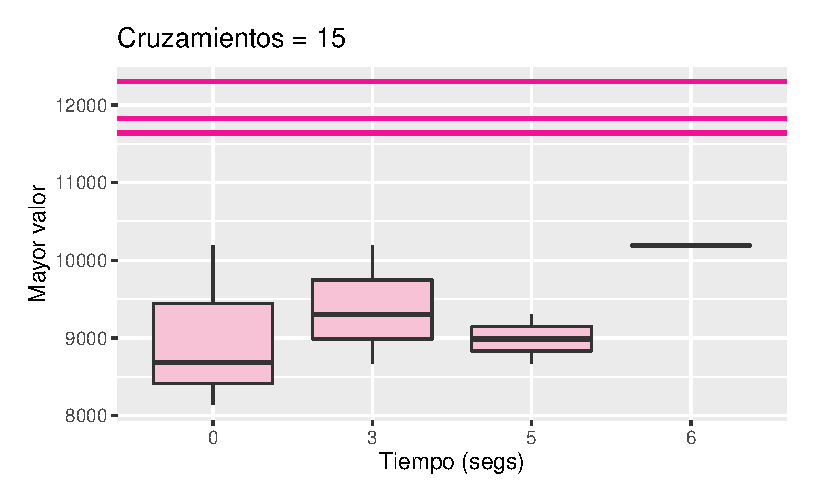
\includegraphics[width=80mm]{R1C15.eps} % archivo
    \caption{Variaci\'on de cruzamientos. Regla 1.}
    \label{Figura 1}
\end{figure}
\begin{figure}[htb] % figura
    \centering
    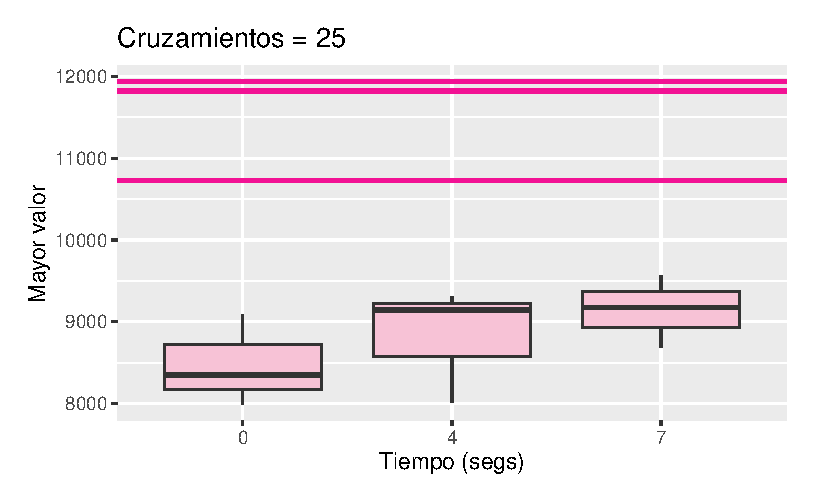
\includegraphics[width=80mm]{R1C25.eps} % archivo
    \caption{Variaci\'on de cruzamientos. Regla 1.}
    \label{Figura 2}
\end{figure}
\begin{figure}[htb] % figura
    \centering
    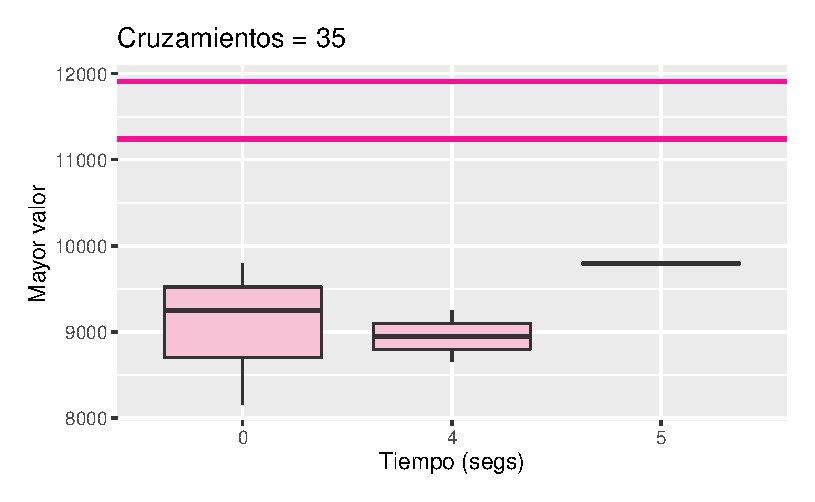
\includegraphics[width=80mm]{R1C35.eps} % archivo
    \caption{Variaci\'on de cruzamientos. Regla 1.}
    \label{Figura 3}
\end{figure}

\begin{figure}[htb] % figura
    \centering
    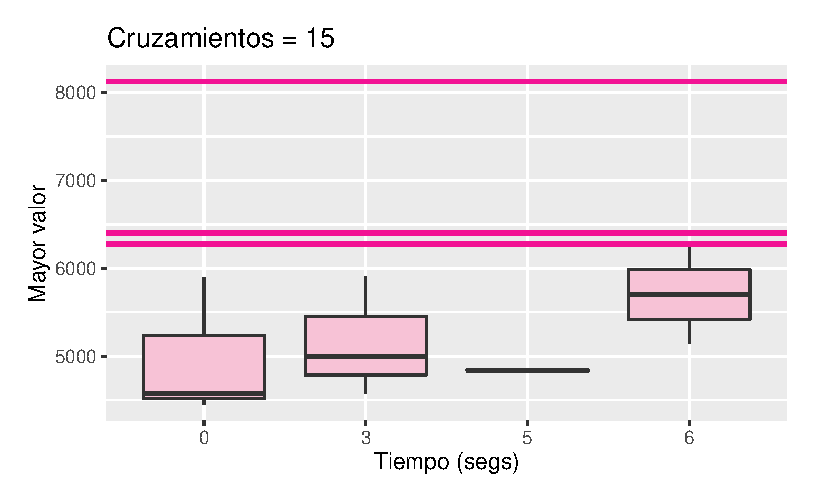
\includegraphics[width=80mm]{R2C15.eps} % archivo
    \caption{Variaci\'on de cruzamientos. Regla 2.}
    \label{Figura 4}
\end{figure}
\begin{figure}[htb] % figura
    \centering
    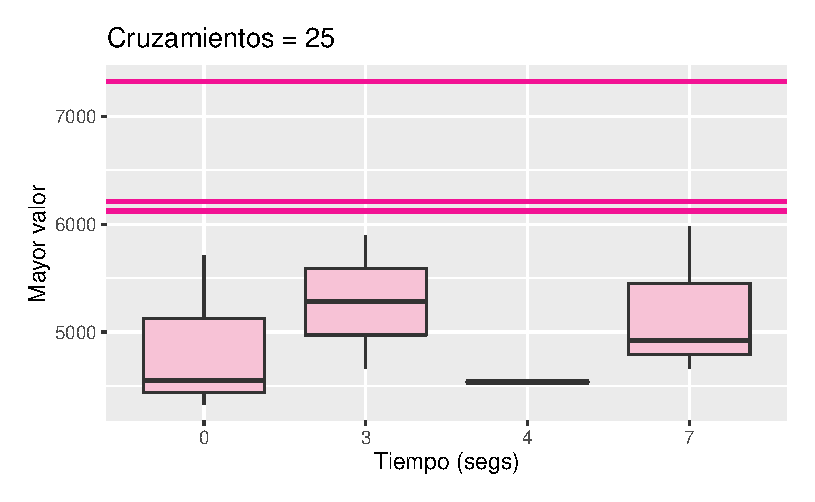
\includegraphics[width=80mm]{R2C25.eps} % archivo
    \caption{Variaci\'on de cruzamientos. Regla 2.}
    \label{Figura 5}
\end{figure}
\begin{figure}[htb] % figura
    \centering
    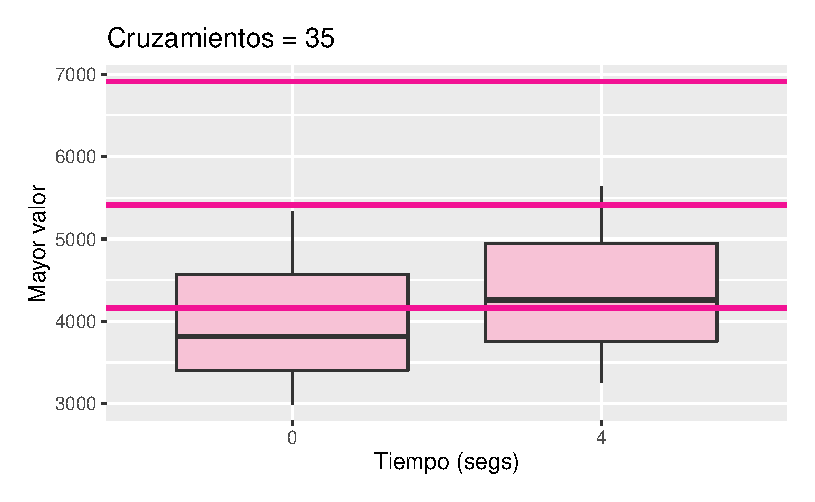
\includegraphics[width=80mm]{R2C35.eps} % archivo
    \caption{Variaci\'on de cruzamientos. Regla 2.}
    \label{Figura 6}
\end{figure}
\begin{figure}[htb] % figura
    \centering
    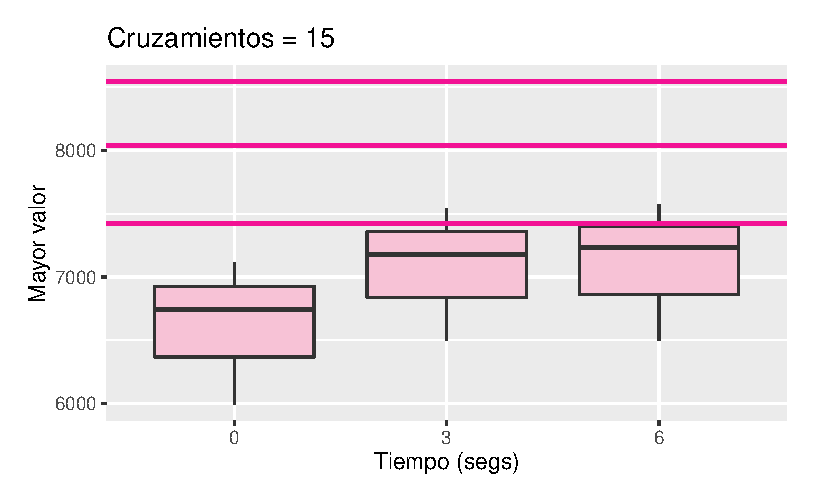
\includegraphics[width=80mm]{R3C15.eps} % archivo
    \caption{Variaci\'on de cruzamientos. Regla 3.}
    \label{Figura 7}
\end{figure}
\begin{figure}[htb] % figura
    \centering
    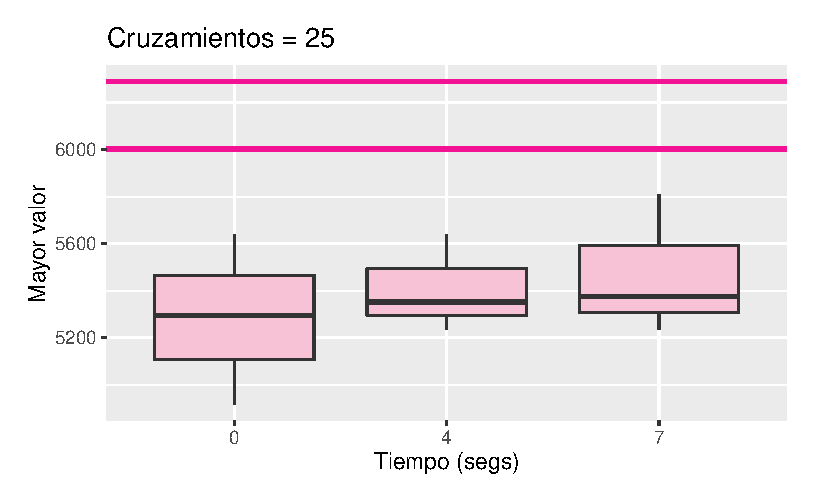
\includegraphics[width=80mm]{R3C25.eps} % archivo
    \caption{Variaci\'on de cruzamientos. Regla 3.}
    \label{Figura 8}
\end{figure}
\begin{figure}[htb] % figura
    \centering
    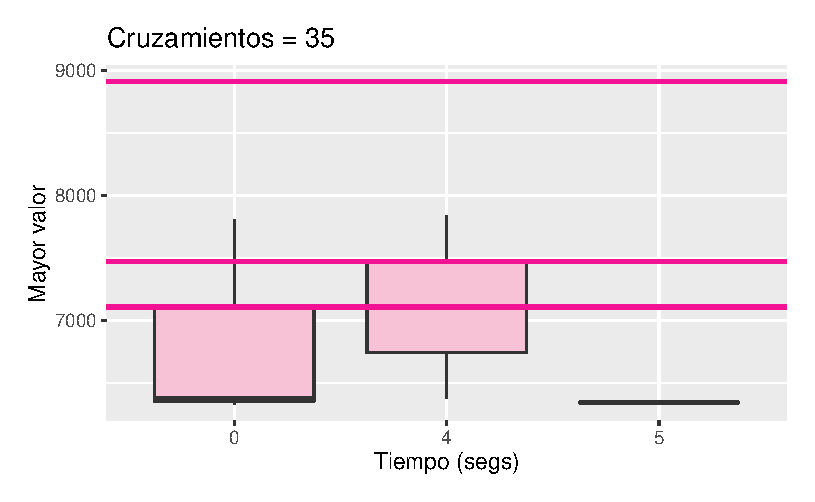
\includegraphics[width=80mm]{R3C35.eps} % archivo
    \caption{Variaci\'on de cruzamientos. Regla 3.}
    \label{Figura 9}
\end{figure}

\newpage
\section{Mutaciones.}
\begin{lstlisting}[language=R, caption= Segmento de c\'odigo Mutaciones.]

mut = c(0.2, 0.5, 0.8) #mutacion
rep <- 10 #cruzamientos
reply = 1:3
for (pm in mut){
  for (replica in reply){
    n <- 50 #objetos
    pesos <- generador.pesos(n, 15, 80)
    valores <- generador.valores(pesos, 10, 500)
    capacidad <- round(sum(pesos) * 0.65)
    optimo <- knapsack(capacidad, pesos, valores)
    init <- 30  #soluciones
    p <- poblacion.inicial(n, init)
    tam <- dim(p)[1]
    assert(tam == init)
    mejores <- double()
    
    tiempo = 8 #segundos
    start = Sys.time()
\end{lstlisting}

\begin{figure}[htb] % figura
    \centering
    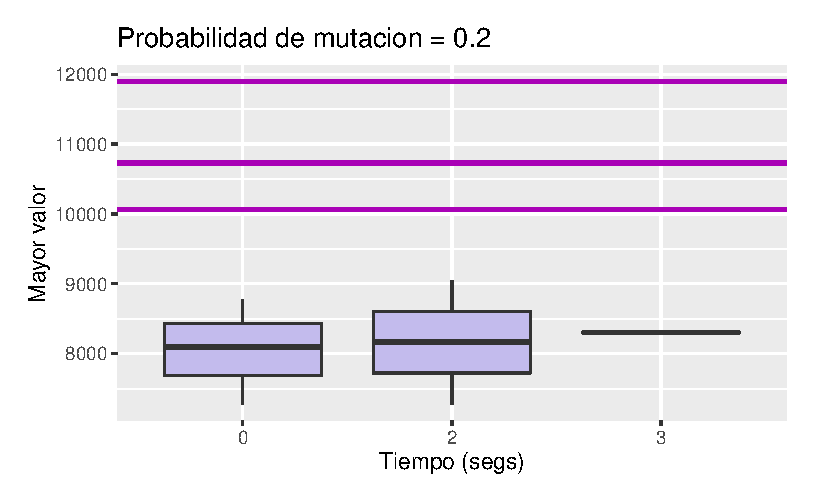
\includegraphics[width=80mm]{R1M2.eps} % archivo
    \caption{Variaci\'on de Mutaciones. Regla 1.}
    \label{Figura 10}
\end{figure}
\begin{figure}[htb] % figura
    \centering
    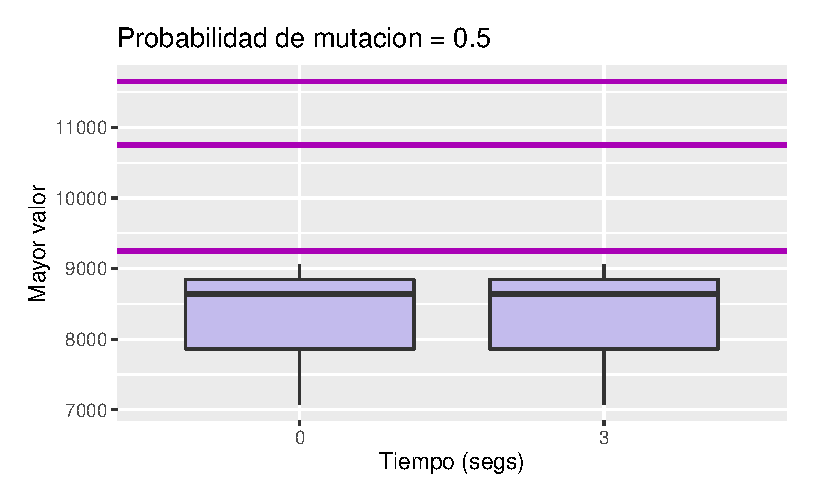
\includegraphics[width=80mm]{R1M5.eps} % archivo
    \caption{Variaci\'on de Mutaciones. Regla 1.}
    \label{Figura 11}
\end{figure}
\begin{figure}[htb] % figura
    \centering
    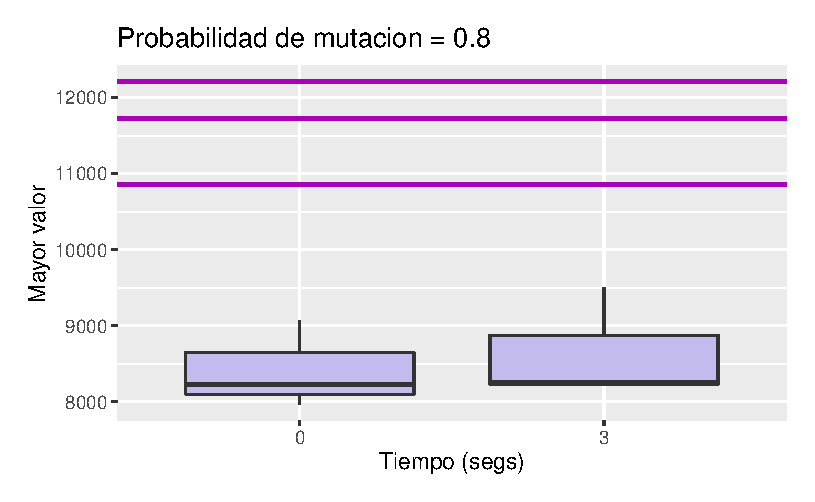
\includegraphics[width=80mm]{R1M8.eps} % archivo
    \caption{Variaci\'on de Mutaciones. Regla 1.}
    \label{Figura 12}
\end{figure}
\begin{figure}[htb] % figura
    \centering
    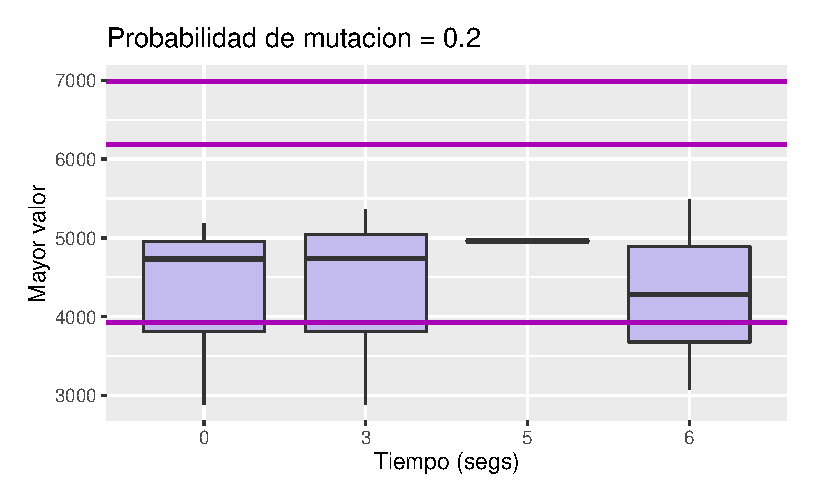
\includegraphics[width=80mm]{R2M2.eps} % archivo
    \caption{Variaci\'on de Mutaciones. Regla 2.}
    \label{Figura 13}
\end{figure}
\begin{figure}[htb] % figura
    \centering
    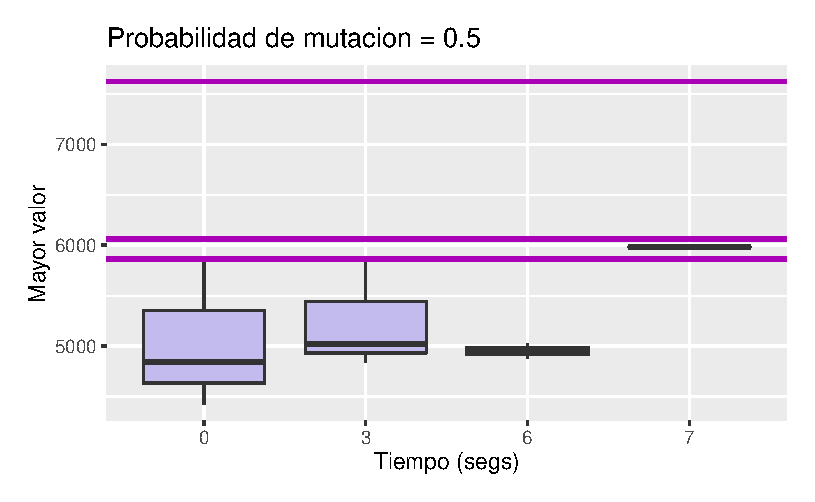
\includegraphics[width=80mm]{R2M5.eps} % archivo
    \caption{Variaci\'on de Mutaciones. Regla 2.}
    \label{Figura 14}
\end{figure}
\begin{figure}[htb] % figura
    \centering
    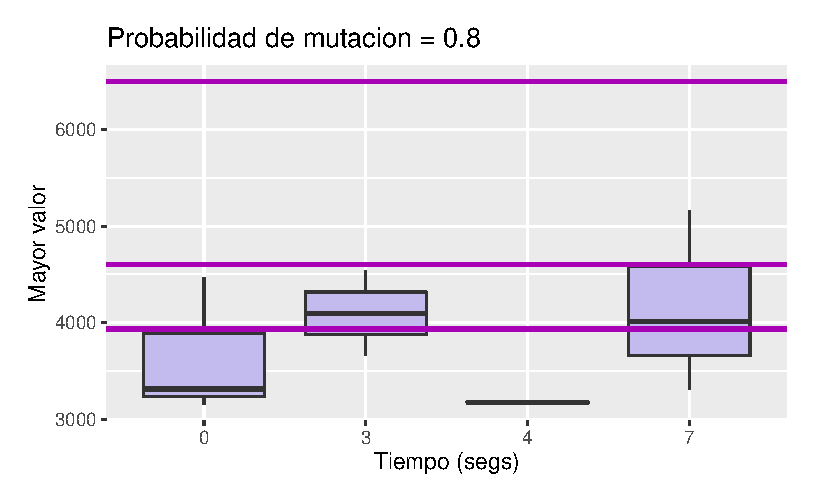
\includegraphics[width=80mm]{R2M8.eps} % archivo
    \caption{Variaci\'on de Mutaciones. Regla 2.}
    \label{Figura 15}
\end{figure}
\begin{figure}[htb] % figura
    \centering
    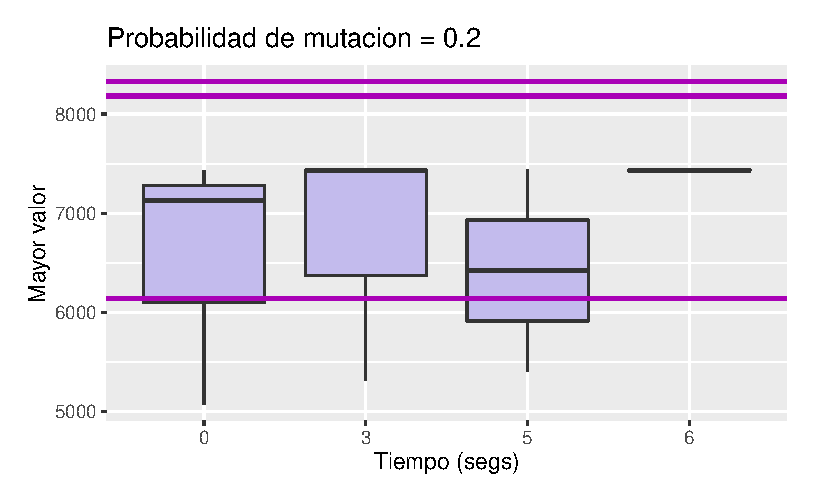
\includegraphics[width=80mm]{R3M2.eps} % archivo
    \caption{Variaci\'on de Mutaciones. Regla 3.}
    \label{Figura 16}
\end{figure}
\begin{figure}[htb] % figura
    \centering
    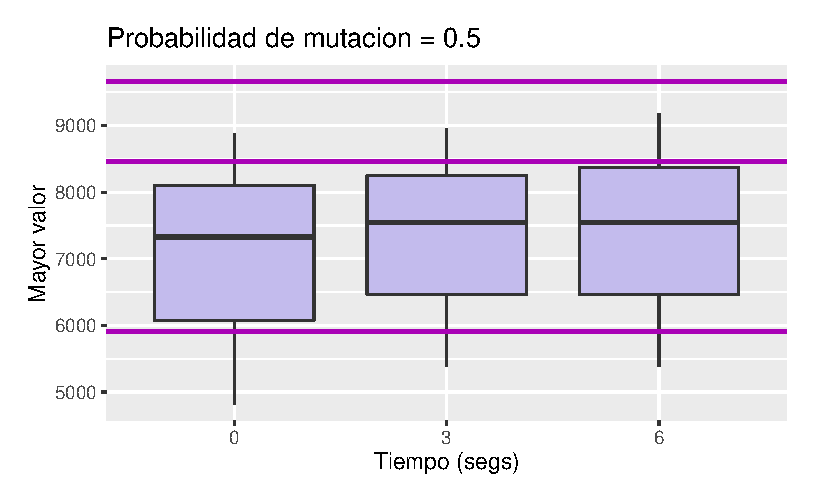
\includegraphics[width=80mm]{R3M5.eps} % archivo
    \caption{Variaci\'on de Mutaciones. Regla 3.}
    \label{Figura 17}
\end{figure}
\begin{figure}[htb] % figura
    \centering
    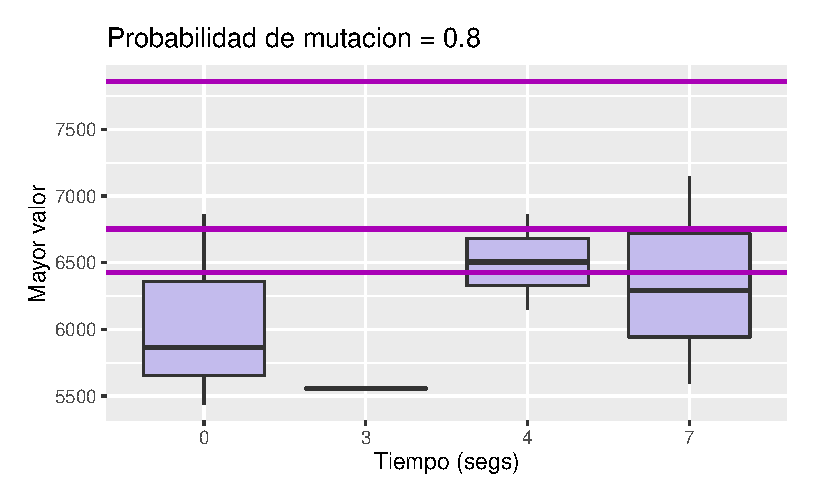
\includegraphics[width=80mm]{R3M8.eps} % archivo
    \caption{Variaci\'on de Mutaciones. Regla 3.}
    \label{Figura 18}
\end{figure}




\section{Poblaciones.}
\begin{lstlisting}[language=R, caption= Segmento de c\'odigo Poblaciones.]

pm = 0.1 #Mutacion
rep <- 15 #Cruzamientos
solu = c(20, 35, 50) #Soluciones
reply = 1:2
for (init in solu){
  for (replica in reply){
    n <- 50 #Objetos
    pesos <- generador.pesos(n, 15, 80)
    valores <- generador.valores(pesos, 10, 500)
    capacidad <- round(sum(pesos) * 0.65)
    optimo <- knapsack(capacidad, pesos, valores)
    p <- poblacion.inicial(n, init)
    tam <- dim(p)[1]
    assert(tam == init)
    mejores <- double()
    
    tiempo = 8 #segundos
    start = Sys.time()
\end{lstlisting}

\begin{figure}[htb] % figura
    \centering
    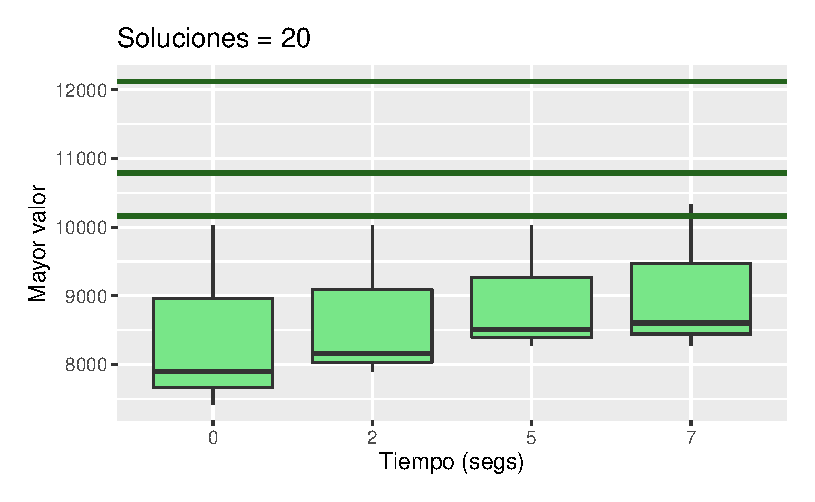
\includegraphics[width=80mm]{R1P20.eps} % archivo
    \caption{Variaci\'on de Poblaciones. Regla 1.}
    \label{Figura 19}
\end{figure}
\begin{figure}[htb] % figura
    \centering
    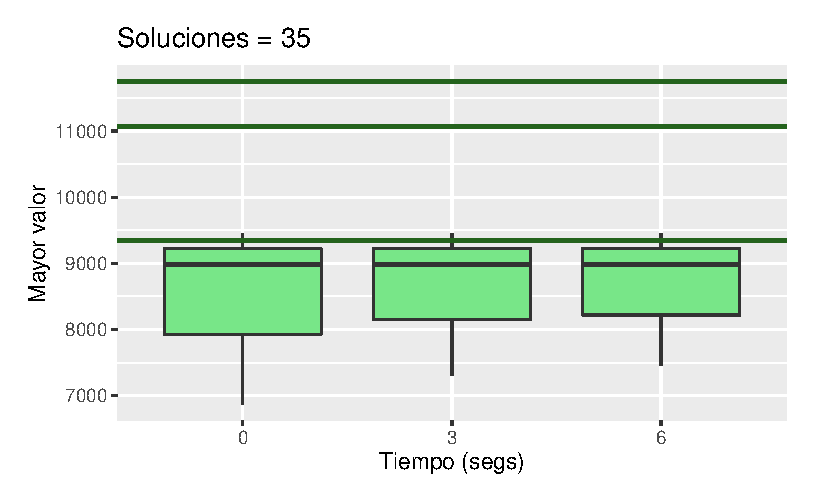
\includegraphics[width=80mm]{R1P35.eps} % archivo
    \caption{Variaci\'on de Poblaciones. Regla 1.}
    \label{Figura 20}
\end{figure}
\begin{figure}[htb] % figura
    \centering
    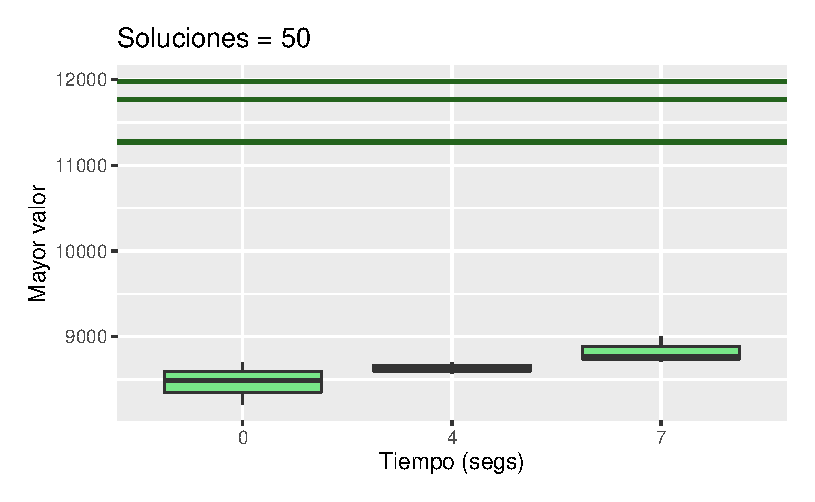
\includegraphics[width=80mm]{R1P50.eps} % archivo
    \caption{Variaci\'on de Poblaciones. Regla 1.}
    \label{Figura 21}
\end{figure}
\begin{figure}[htb] % figura
    \centering
    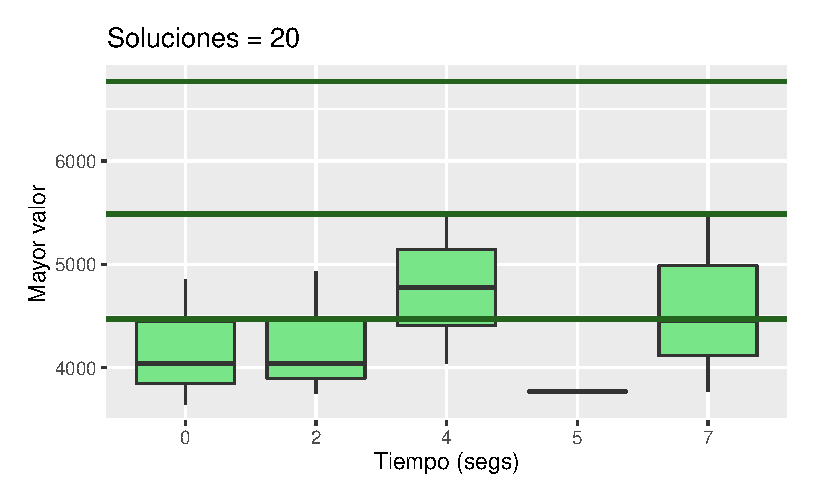
\includegraphics[width=80mm]{R2P20.eps} % archivo
    \caption{Variaci\'on de Poblaciones. Regla 2.}
    \label{Figura 22}
\end{figure}
\begin{figure}[htb] % figura
    \centering
    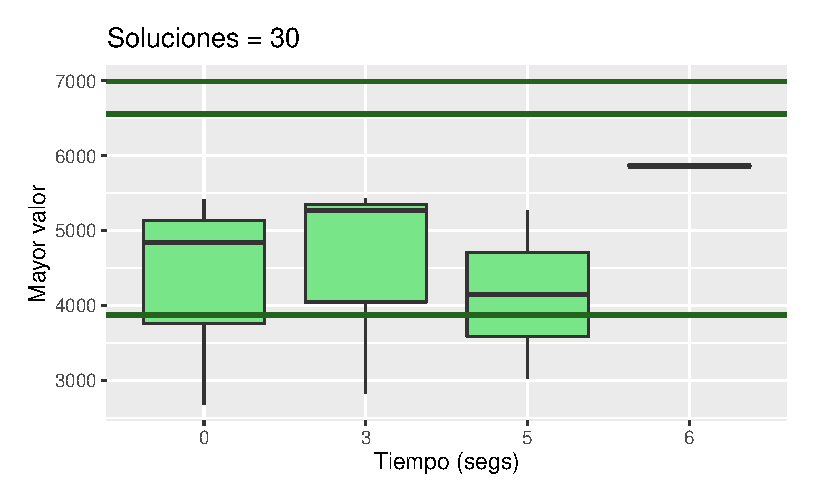
\includegraphics[width=80mm]{R2P30.eps} % archivo
    \caption{Variaci\'on de Poblaciones. Regla 2.}
    \label{Figura 23}
\end{figure}
\begin{figure}[htb] % figura
    \centering
    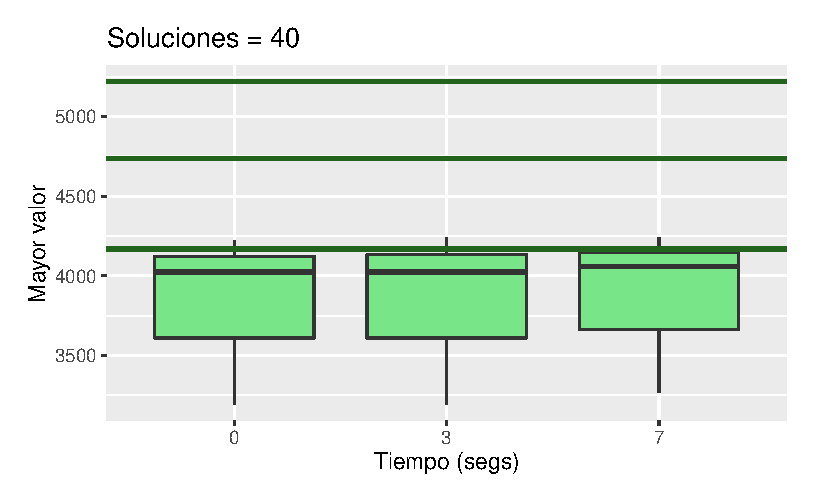
\includegraphics[width=80mm]{R2P40.eps} % archivo
    \caption{Variaci\'on de Poblaciones. Regla 2.}
    \label{Figura 24}
\end{figure}
\begin{figure}[htb] % figura
    \centering
    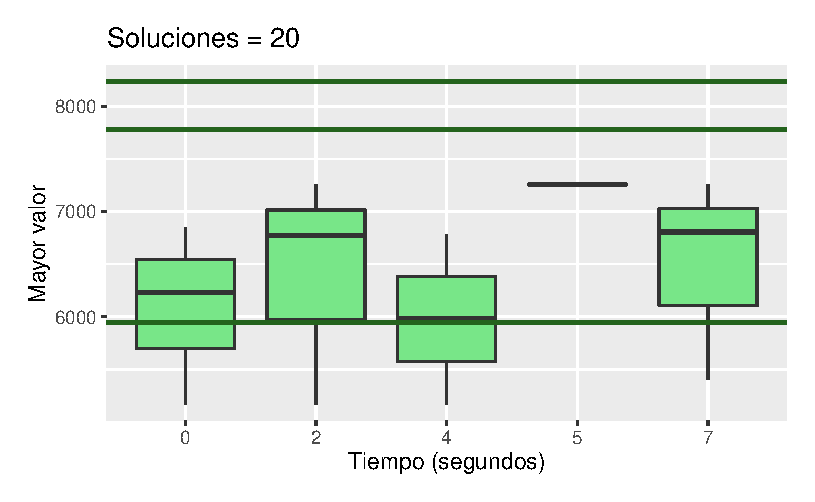
\includegraphics[width=80mm]{R3P20.eps} % archivo
    \caption{Variaci\'on de Poblaciones. Regla 3.}
    \label{Figura 25}
\end{figure}
\begin{figure}[htb] % figura
    \centering
    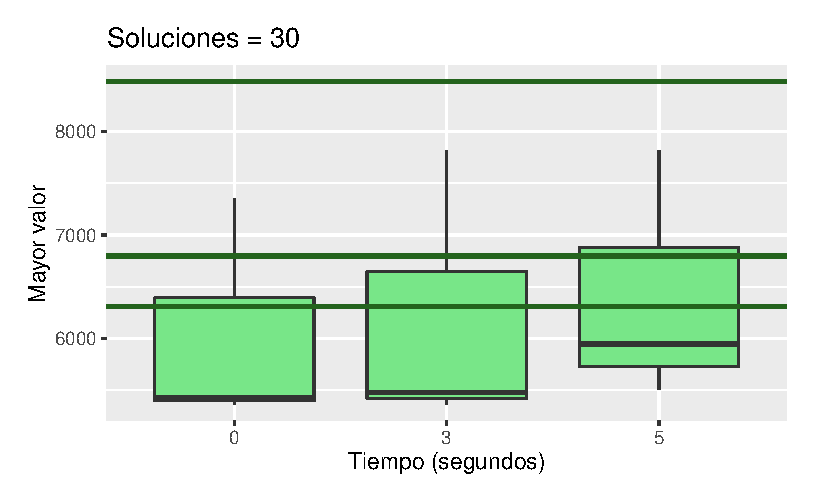
\includegraphics[width=80mm]{R3P30.eps} % archivo
    \caption{Variaci\'on de Poblaciones. Regla 3.}
    \label{Figura 26}
\end{figure}
\begin{figure}[htb] % figura
    \centering
    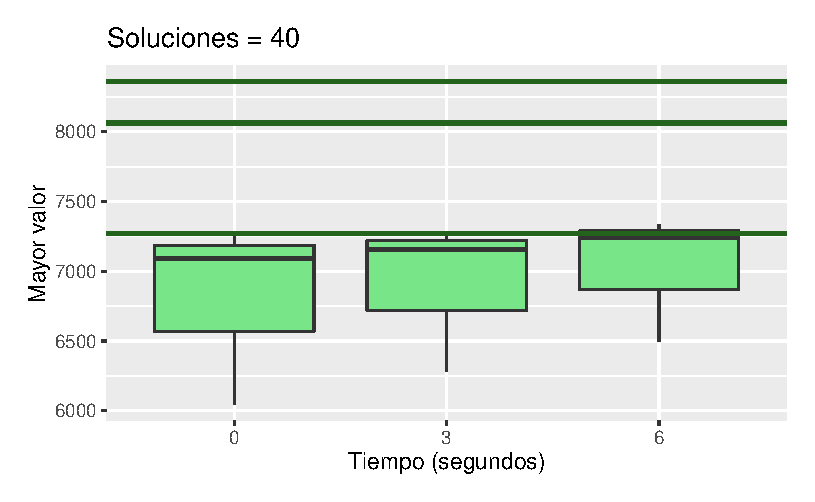
\includegraphics[width=80mm]{R3P40.eps} % archivo
    \caption{Variaci\'on de Poblaciones. Regla 3.}
    \label{Figura 27}
\end{figure}



\newpage

\section{Estad\'istica.}

\begin{table}[ht]
    \centering
    \caption{Resultados obtenidos de prueba de normalidad de Shapiro. Regla 1 Cruzamiento.} 
    \begin{tabular}{|c|c|c|c|}
    \hline
    Carga & W value & P value & ¿Se acepta H0?  \\
    \hline
    15 & 0.8682 & 0.1177 & s\'i \\
    \hline 
     25 & 0.9009 & 0.2578 & s\'i  \\
    \hline 
    35 & 0.9053 & 0.0462 & no \\
    \hline 
\end{tabular}
    \label{cuadro 1}
\end{table}

\begin{table}[htb]
    \centering
    \caption{Diferencias entre grupos. Kruskal-Wallis. Regla 1 Cruzamiento.} 
    \begin{tabular}{|c|c|c|}
    \hline
    "" & 15 & 25 \\
    \hline
    25 & 0.79 & ""  \\
    \hline
    35 & 0.79 & 0.79  \\
    \hline
\end{tabular}
    \label{cuadro 2}
\end{table}

\begin{table}[htb]
    \centering
    \caption{Informaci\'on individual de los datos. Regla 1 Cruzamiento.} 
    \begin{tabular}{|c|c|c|c|c|c|c|}
    \hline
    Carga & Qty. Participantes & promedio & Desv. Std. & Varianza & Mediana & Rango Intercuartil  \\
    \hline
    15 & 9 & 9262 & 780 & 608886 & 9301 & 1520 \\
    \hline
    5 & 9 & 8813 & 579 & 335060 & 9093 & 825 \\
    \hline
    35 & 6 & 9150 & 645 & 415876 & 9249 & 859 \\
    \hline
\end{tabular}
    \label{cuadro 3}
\end{table}



\begin{table}[ht]
    \centering
    \caption{Resultados obtenidos de prueba de normalidad de Shapiro. Regla 2 Cruzamiento.} 
    \begin{tabular}{|c|c|c|c|}
    \hline
    Carga & W value & P value & ¿Se acepta H0?  \\
    \hline
    15 & 0.8807 & 0.16 & s\'i \\
    \hline 
     25 & 0.8267 & 0.04 &  no \\
    \hline 
    35 & 0.9223 & 0.52 & s\'i \\
    \hline 
\end{tabular}
    \label{cuadro 4}
\end{table}

\begin{table}[htb]
    \centering
    \caption{Diferencias entre grupos. Kruskal-Wallis. Regla 2 Cruzamiento.} 
    \begin{tabular}{|c|c|c|}
    \hline
    "" & 15 & 25 \\
    \hline
    25 & 0.48 & ""  \\
    \hline
    35 & 0.26 & 0.26  \\
    \hline
\end{tabular}
    \label{cuadro 5}
\end{table}

\begin{table}[htb]
    \centering
    \caption{Informaci\'on individual de los datos. Regla 2 Cruzamiento.} 
    \begin{tabular}{|c|c|c|c|c|c|c|}
    \hline
    Carga & Qty. Participantes & promedio & Desv. Std. & Varianza & Mediana & Rango Intercuartil  \\
    \hline
    15 & 15 & 5185 & 673 & 452995 & 5001 & 1324 \\
    \hline
    5 & 25 & 5028 & 648 & 419847 & 4666 & 1158 \\
    \hline
    35 & 35 & 4216 & 1080 & 1167110 & 4036 & 1666 \\
    \hline
\end{tabular}
    \label{cuadro 6}
\end{table}



\begin{table}[ht]
    \centering
    \caption{Resultados obtenidos de prueba de normalidad de Shapiro. Regla 3 Cruzamiento.} 
    \begin{tabular}{|c|c|c|c|}
    \hline
    Carga & W value & P value & ¿Se acepta H0?  \\
    \hline
    15 & 0.9372 & 0.5534 & s\'i \\
    \hline 
     25 & 0.9511 & 0.7029 &  s\'i \\
    \hline 
    35 & 0.6631 & 0.0024 & no \\
    \hline 
\end{tabular}
    \label{cuadro 7}
\end{table}

\begin{table}[htb]
    \centering
    \caption{Diferencias entre grupos. Kruskal-Wallis. Regla 3 Cruzamiento.} 
    \begin{tabular}{|c|c|c|}
    \hline
    "" & 15 & 25 \\
    \hline
    25 & 0.0012 & ""  \\
    \hline
    35 & 0.5952 & 0.0035  \\
    \hline
\end{tabular}
    \label{cuadro 8}
\end{table}

\begin{table}[htb]
    \centering
    \caption{Informaci\'on individual de los datos. Regla 3 Cruzamiento.} 
    \begin{tabular}{|c|c|c|c|c|c|c|}
    \hline
    Carga & Qty. Participantes & promedio & Desv. Std. & Varianza & Mediana & Rango Intercuartil  \\
    \hline
    15 & 15 & 6929 & 530 & 281256 & 7112 & 735 \\
    \hline
    5 & 25 & 5389 & 269 & 72359 & 5353 & 402 \\
    \hline
    35 & 35 & 6848 & 758 & 574169 & 6378 & 1100 \\
    \hline
\end{tabular}
    \label{cuadro 9}
\end{table}



\begin{table}[ht]
    \centering
    \caption{Resultados obtenidos de prueba de normalidad de Shapiro. Regla 1 Mutacion.} 
    \begin{tabular}{|c|c|c|c|}
    \hline
    Carga & W value & P value & ¿Se acepta H0?  \\
    \hline
    0.2 & 0.9268 & 0.4159 & s\'i \\
    \hline 
     0.5 & 0.7675 & 0.0294 &  no \\
    \hline 
    0.8 & 0.8249 & 0.0972 & s\'i \\
    \hline 
\end{tabular}
    \label{cuadro 10}
\end{table}

\begin{table}[htb]
    \centering
    \caption{Diferencias entre grupos. Kruskal-Wallis. Regla 1 Mutacion.} 
    \begin{tabular}{|c|c|c|}
    \hline
    "" & 0.2 & 0.5 \\
    \hline
    0.5 & 1 & ""  \\
    \hline
    0.8 & 1 & 1  \\
    \hline
\end{tabular}
    \label{cuadro 11}
\end{table}

\begin{table}[htb]
    \centering
    \caption{Informaci\'on individual de los datos. Regla 1 Mutacion.} 
    \begin{tabular}{|c|c|c|c|c|c|c|}
    \hline
    Carga & Qty. Participantes & promedio & Desv. Std. & Varianza & Mediana & Rango Intercuartil  \\
    \hline
    0.2 & 6 & 8130 & 741 & 549403 & 8198 & 1174 \\
    \hline
    0.5 & 6 & 8258 & 931 & 866729 & 8639 & 1480 \\
    \hline
    0.8 & 6 & 8542 & 602 & 362304 & 8238 & 634 \\
    \hline
\end{tabular}
    \label{cuadro 12}
\end{table}




\begin{table}[ht]
    \centering
    \caption{Resultados obtenidos de prueba de normalidad de Shapiro. Regla 2 Mutacion.} 
    \begin{tabular}{|c|c|c|c|}
    \hline
    Carga & W value & P value & ¿Se acepta H0?  \\
    \hline
    0.2 & 0.8026 & 0.0219 & no \\
    \hline 
     0.5 & 0.8504 & 0.0752 &  s\'i \\
    \hline 
    0.8 & 0.8859 & 0.1813 & s\'i \\
    \hline 
\end{tabular}
    \label{cuadro 13}
\end{table}

\begin{table}[htb]
    \centering
    \caption{Diferencias entre grupos. Kruskal-Wallis. Regla 2 Mutacion.} 
    \begin{tabular}{|c|c|c|}
    \hline
    "" & 0.2 & 0.5 \\
    \hline
    0.5 & 0.31 & ""  \\
    \hline
    0.8 & 0.37 & 0.01  \\
    \hline
\end{tabular}
    \label{cuadro 14}
\end{table}

\begin{table}[htb]
    \centering
    \caption{Informaci\'on individual de los datos. Regla 2 Mutacion.} 
    \begin{tabular}{|c|c|c|c|c|c|c|}
    \hline
    Carga & Qty. Participantes & promedio & Desv. Std. & Varianza & Mediana & Rango Intercuartil  \\
    \hline
    0.2 & 9 & 4370 & 1092 & 1191416 & 4736 & 2107 \\
    \hline
    0.5 & 9 & 5194 & 562 & 315869 & 5021 & 1027 \\
    \hline
    0.8 & 9 & 3866 & 719 & 517514 & 3660 & 1164 \\
    \hline
\end{tabular}
    \label{cuadro 15}
\end{table}



\begin{table}[ht]
    \centering
    \caption{Resultados obtenidos de prueba de normalidad de Shapiro. Regla 3 Mutacion.} 
    \begin{tabular}{|c|c|c|c|}
    \hline
    Carga & W value & P value & ¿Se acepta H0?  \\
    \hline
    0.2 & 0.6922 & 0.0011 & no \\
    \hline 
     0.5 & 0.8819 & 0.1645 &  s\'i \\
    \hline 
    0.8 & 0.9093 & 0.3116 & s\'i \\
    \hline 
\end{tabular}
    \label{cuadro 16}
\end{table}

\begin{table}[htb]
    \centering
    \caption{Diferencias entre grupos. Kruskal-Wallis. Regla 3 Mutacion.} 
    \begin{tabular}{|c|c|c|}
    \hline
    "" & 0.2 & 0.5 \\
    \hline
    0.5 & 0.75 & ""  \\
    \hline
    0.8 & 0.75 & 0.75  \\
    \hline
\end{tabular}
    \label{cuadro 17}
\end{table}

\begin{table}[htb]
    \centering
    \caption{Informaci\'on individual de los datos. Regla 3 Mutacion.} 
    \begin{tabular}{|c|c|c|c|c|c|c|}
    \hline
    Carga & Qty. Participantes & promedio & Desv. Std. & Varianza & Mediana & Rango Intercuartil  \\
    \hline
    0.2 & 9 & 6676 & 1067 & 1137428 & 7430 & 2028 \\
    \hline
    0.5 & 9 & 7224 & 1671 & 2792608 & 7549 & 3498 \\
    \hline
    0.8 & 9 & 6195 & 637 & 405675 & 6148 & 1263 \\
    \hline
\end{tabular}
    \label{cuadro 18}
\end{table}




\begin{table}[ht]
    \centering
    \caption{Resultados obtenidos de prueba de normalidad de Shapiro. Regla 1 Poblacion.} 
    \begin{tabular}{|c|c|c|c|}
    \hline
    Carga & W value & P value & ¿Se acepta H0?  \\
    \hline
    20 & 0.8581 & 0.0463 & no \\
    \hline 
     35 & 0.7943 & 0.0175 &  no \\
    \hline 
    50 & 0.9402 & 0.5844 & s\'i \\
    \hline 
\end{tabular}
    \label{cuadro 19}
\end{table}

\begin{table}[htb]
    \centering
    \caption{Diferencias entre grupos. Kruskal-Wallis. Regla 1 Poblacion.} 
    \begin{tabular}{|c|c|c|}
    \hline
    "" & 20 & 35 \\
    \hline
    35 & 1 & ""  \\
    \hline
    50 & 1 & 1  \\
    \hline
\end{tabular}
    \label{cuadro 20}
\end{table}

\begin{table}[htb]
    \centering
    \caption{Informaci\'on individual de los datos. Regla 1 Poblacion.} 
    \begin{tabular}{|c|c|c|c|c|c|c|}
    \hline
    Carga & Qty. Participantes & promedio & Desv. Std. & Varianza & Mediana & Rango Intercuartil  \\
    \hline
    20 & 12 & 8788 & 1019 & 1037725 & 8396 & 1928 \\
    \hline
    35 & 9 & 8550 & 1036 & 1072658 & 8987 & 2004 \\
    \hline
    50 & 9 & 8643 & 216 & 46642 & 8702 & 145 \\
    \hline
\end{tabular}
    \label{cuadro 21}
\end{table}






\begin{table}[ht]
    \centering
    \caption{Resultados obtenidos de prueba de normalidad de Shapiro. Regla 2 Poblacion.} 
    \begin{tabular}{|c|c|c|c|}
    \hline
    Carga & W value & P value & ¿Se acepta H0?  \\
    \hline
    20 & 0.8530 & 0.0400 & no \\
    \hline 
     35 & 0.7951 & 0.0179 &  no \\
    \hline 
    50 & 0.7557 & 0.0063 & no \\
    \hline 
\end{tabular}
    \label{cuadro 22}
\end{table}

\begin{table}[htb]
    \centering
    \caption{Diferencias entre grupos. Kruskal-Wallis. Regla 2 Poblacion.} 
    \begin{tabular}{|c|c|c|}
    \hline
    "" & 20 & 35 \\
    \hline
    35 & 0.70 & ""  \\
    \hline
    50 & 0.64 & 0.64  \\
    \hline
\end{tabular}
    \label{cuadro 23}
\end{table}

\begin{table}[htb]
    \centering
    \caption{Informaci\'on individual de los datos. Regla 2 Poblacion.} 
    \begin{tabular}{|c|c|c|c|c|c|c|}
    \hline
    Carga & Qty. Participantes & promedio & Desv. Std. & Varianza & Mediana & Rango Intercuartil  \\
    \hline
    20 & 12 & 4361 & 681 & 463701 & 4040 & 1104 \\
    \hline
    35 & 9 & 4517 & 1281 & 1641595 & 5272 & 2391 \\
    \hline
    50 & 9 & 3830 & 468 & 218868 & 4025 & 957 \\
    \hline
\end{tabular}
    \label{cuadro 24}
\end{table}




\begin{table}[ht]
    \centering
    \caption{Resultados obtenidos de prueba de normalidad de Shapiro. Regla 3 Poblacion.} 
    \begin{tabular}{|c|c|c|c|}
    \hline
    Carga & W value & P value & ¿Se acepta H0?  \\
    \hline
    20 & 0.8125 & 0.0130 & no \\
    \hline 
     35 & 0.7389 & 0.0040 &  no \\
    \hline 
    50 & 0.7960 & 0.0184 & no \\
    \hline 
\end{tabular}
    \label{cuadro 25}
\end{table}

\begin{table}[htb]
    \centering
    \caption{Diferencias entre grupos. Kruskal-Wallis. Regla 3 Poblacion.} 
    \begin{tabular}{|c|c|c|}
    \hline
    "" & 20 & 35 \\
    \hline
    35 & 0.80 & ""  \\
    \hline
    50 & 0.33 & 0.50  \\
    \hline
\end{tabular}
    \label{cuadro 26}
\end{table}

\begin{table}[htb]
    \centering
    \caption{Informaci\'on individual de los datos. Regla 3 Poblacion.} 
    \begin{tabular}{|c|c|c|c|c|c|c|}
    \hline
    Carga & Qty. Participantes & promedio & Desv. Std. & Varianza & Mediana & Rango Intercuartil  \\
    \hline
    20 & 12 & 6344 & 871 & 759430 & 6779 & 1605 \\
    \hline
    35 & 9 & 6229 & 1096 & 1201556 & 5507 & 1930 \\
    \hline
    50 & 9 & 6912 & 497 & 246937 & 7155 & 791 \\
    \hline
\end{tabular}
    \label{cuadro 27}
\end{table}








\begin{table}[ht]
    \centering
    \caption{Resultados obtenidos de prueba Kruskal-Wallis.} 
    \begin{tabular}{|c|c|c|c|}
    \hline
    "" & Chi cuadrada & DF & P  \\
    \hline
    RC1 & 1.89 & 2 & 0.3876 \\
    \hline
    RC2 & 4.32 & 2 & 0.1152 \\
    \hline
    RC3 & 4.32 & 2 & 0.1152 \\
    \hline
    RM1 & 0.5760 & 2 & 0.7497 \\
    \hline
    RM2 & 7.5683 & 2 & 0.0227 \\
    \hline
    RM3 & 2.3881 & 2 & 0.3030 \\
    \hline
    RP1 & 0.0827 & 2 & 0.9595 \\
    \hline
    RP2 & 2.1273 & 2 & 0.3452 \\
    \hline
    RP3 & 2.8296 & 2 & 0.2430 \\
    \hline
\end{tabular}
    \label{cuadro 28}
\end{table}
\newpage
%CONCLUSIOOOON
\section{Conclusi\'on.}
Como se mencionó con anterioridad, manteniendo fijo el tiempo en 8 segundos, y con la informaci\'on presentada y resumida en el cuadro \ref{cuadro 28} y en las figuras anteriores, podemos observar que en la \texttt{regla 1}, tanto para \texttt{mutaci\'on, cruzaci\'on y poblaci\'on}. Se logran mejores resultado conforme aumenta el tiempo. 

Para la \texttt{regla 2}, para cruzamientos sucede los mismo que en la regla 1, se obtienen mejores resultados conforme aumenta el tiempo, pero en mutaci\'on no parece existir una relaci\'on signifcativa con el tiempo.

Para la \texttt{regla 3}, para la probabilidad de cruzamiento igual que en la regla \texttt{1}, se observa una tendencia a obtener resultados \'optimos conforme el tiempo avanza. Para la probabilidad de mutaci\'on y de poblaci\'on se presenta la misma situaci'on, mejores resultados proporcionales al tiempo.

Tambien concluimos que existe un diferencia significativa entre las medias de las variables para la regla 1, 2 y 3.
% BIBLIOGRAFIAAAAAAS
\bibliography{referencias}
\bibliographystyle{plainnat}
\end{document}


